\documentclass[11pt,paper=a4,answers]{exam}
\usepackage{graphicx,lastpage}
\usepackage{upgreek}
\usepackage{censor}
\usepackage{gensymb}
\usepackage{amsmath}
\usepackage{multicol}
\usepackage{enumitem}
 \usepackage{pgfplots}
\pgfplotsset{compat=1.18}
\usepackage{tasks}
\usepackage{adjustbox}
\usepackage{xcolor}
\usepackage{tfrupee}
\setlength{\voffset}{0.25in}
\usepackage{tabularx}
\newcolumntype{Y}{>{\centering\arraybackslash}X}
%==============================================================
% Customise Non-Essential Packages Below
% =============================================================
\usepackage[most]{tcolorbox}
\usepackage{eso-pic}
\usepackage{tikz}
\AddToShipoutPictureBG{%
\begin{tikzpicture}[remember picture,overlay]
\foreach \x in {-8,-4,0,4,8,12,16,20}
\foreach \y in {-8,-4,0,4,8,12,16,20} {
\node[opacity=0.05,rotate=45,anchor=center] at ([xshift=\x cm,yshift=\y cm]current page.center) {%
\begin{minipage}{2cm}
\centering
\includegraphics[width=2cm]{images/logo_black.png}\\
\small preppeo.com
\end{minipage}%
};
}
\end{tikzpicture}%
}
\printanswers

%==============================================================
% Customise Non-Essential Packages Above
% =============================================================
\definecolor{svgray}{rgb}{0.90, 0.90, 0.90}
\graphicspath{{images/}}

\usepackage[normalem]{ulem}
\renewcommand\ULthickness{1pt}   %%---> For changing thickness of underline
\setlength\ULdepth{3.5ex}%\maxdimen ---> For changing depth of underline
\renewcommand{\baselinestretch}{1}
\chead{
\includegraphics[scale=0.1,height=2cm ]{logo.png}
}
\pagestyle{empty}

\pagestyle{headandfoot}
\headrule
\cfoot{W: https://preppeo.com; M: +91-8130711689}

\begin{document}
%==============================================================
% Customise Question paper details below this
% =============================================================
\begin{center}
    \centering
    \renewcommand{\arraystretch}{1.5}
    \begin{tabularx}{\textwidth}{YYY}
    & \normalsize\bf{{\Large{{Quantitative Reasoning}}}} & \\
    By Preppeo & \normalsize\bf{MOCK } & GRE\\
    \normalsize{\textbf{Questions:} 15 (Section 2 : 15} & \normalsize{\textbf{Marks:} 15 } & \normalsize{\textbf{Time:}  minutes } \\
    \end{tabularx}
\end{center}
\par\noindent\rule{\textwidth}{1pt}
% =============================================================
% Customise Question paper details above this
% =============================================================

\begin{questions}
\pointsinrightmargin
\pointsdroppedatright
\marksnotpoints
\pointpoints{mark}{marks}
\pointformat{\boldmath\themarginpoints}
\bracketedpoints

% =============================================================
% Question Begin
% =============================================================

\section*{Section 2 - Mock 2 Set 2 (Easy)}

% --- QUANTITY COMPARISON (5 QUESTIONS) ---

%Q: 1
\question
\textbf{Quantity A: } $\dfrac{1}{4} + \dfrac{1}{5} + \dfrac{1}{6}$ \\
\vspace{5pt}
\textbf{Quantity B: } 0.6

\begin{tasks}(1)
\task[A)] Quantity A is greater
\task[B)] Quantity B is greater
\task[C)] The two quantities are equal
\task[D)] The relationship cannot be determined
\end{tasks}

\begin{solution}
To compare these quantities, we first find a common denominator for the fractions in Quantity A.
\vspace{5pt}
\begin{center}
The least common multiple of 4, 5, and 6 is 60.
\vspace{5pt}
$\dfrac{15}{60} + \dfrac{12}{60} + \dfrac{10}{60} = \dfrac{37}{60}$
\vspace{5pt}
Convert the fraction to a decimal: $37 \div 60 \approx 0.616$
\end{center}
\vspace{5pt}
Comparing 0.616 (Quantity A) to 0.6 (Quantity B), Quantity A is greater.

Answer: \colorbox{yellow!100}{A}
\end{solution}

\vspace{1cm}

%Q: 2
\question
\begin{center}
\begin{tikzpicture}
    \draw[thick] (0,0) -- (4,0) -- (1,2) -- cycle;
    \node at (0.5, 0.2) {$x^\circ$};
    \node at (3.5, 0.2) {$y^\circ$};
    \node[above] at (1,2) {$z^\circ$};
\end{tikzpicture}
\end{center}
In the triangle above, $x + y = 130$.
\vspace{5pt}
\textbf{Quantity A: } $z$ \\
\vspace{5pt}
\textbf{Quantity B: } 50

\begin{tasks}(1)
\task[A)] Quantity A is greater
\task[B)] Quantity B is greater
\task[C)] The two quantities are equal
\task[D)] The relationship cannot be determined
\end{tasks}

\begin{solution}
The sum of the interior angles of a triangle is always $180^\circ$.
\vspace{5pt}
\begin{center}
$x + y + z = 180$
\vspace{5pt}
Substitute $130$ for $x + y$:
\vspace{5pt}
$130 + z = 180 \implies z = 50$
\end{center}
\vspace{5pt}
Since Quantity A is 50 and Quantity B is 50, they are equal.

Answer: \colorbox{yellow!100}{C}
\end{solution}

\vspace{1cm}

%Q: 3
\question
$x$ is an integer such that $x^2 - 5x + 6 = 0$.
\vspace{5pt}
\textbf{Quantity A: } $x$ \\
\vspace{5pt}
\textbf{Quantity B: } 2.5

\begin{tasks}(1)
\task[A)] Quantity A is greater
\task[B)] Quantity B is greater
\task[C)] The two quantities are equal
\task[D)] The relationship cannot be determined
\end{tasks}

\begin{solution}
First, solve the quadratic equation by factoring:
\vspace{5pt}
\begin{center}
$(x - 2)(x - 3) = 0$
\vspace{5pt}
The possible values for $x$ are $2$ or $3$.
\end{center}
\vspace{5pt}
If $x = 2$, Quantity B is greater. If $x = 3$, Quantity A is greater.
\vspace{5pt}
Because the relationship depends on which value of $x$ is chosen, it cannot be determined.

Answer: \colorbox{yellow!100}{D}
\end{solution}

\vspace{1cm}

%Q: 4
\question
\textbf{Quantity A: } The number of distinct prime factors of 120 \\
\vspace{5pt}
\textbf{Quantity B: } The number of distinct prime factors of 150

\begin{tasks}(1)
\task[A)] Quantity A is greater
\task[B)] Quantity B is greater
\task[C)] The two quantities are equal
\task[D)] The relationship cannot be determined
\end{tasks}

\begin{solution}
Perform the prime factorization for both numbers:
\vspace{5pt}
\begin{center}
$120 = 12 \times 10 = (2^2 \times 3) \times (2 \times 5) = 2^3 \times 3 \times 5$ \\
Distinct factors: $\{2, 3, 5\}$ (Count = 3)
\vspace{10pt}
$150 = 15 \times 10 = (3 \times 5) \times (2 \times 5) = 2 \times 3 \times 5^2$ \\
Distinct factors: $\{2, 3, 5\}$ (Count = 3)
\end{center}
\vspace{5pt}
Both quantities are equal.

Answer: \colorbox{yellow!100}{C}
\end{solution}

\vspace{1cm}

%Q: 5
\question
Child A ate 3/5 of a 1kg cake. Child B ate 450 grams of the same cake.
\vspace{5pt}
\textbf{Quantity A: } Weight eaten by Child A \\
\vspace{5pt}
\textbf{Quantity B: } Weight eaten by Child B

\begin{tasks}(1)
\task[A)] Quantity A is greater
\task[B)] Quantity B is greater
\task[C)] The two quantities are equal
\task[D)] The relationship cannot be determined
\end{tasks}

\begin{solution}
Convert both quantities to the same unit (grams).
\vspace{5pt}
\begin{center}
$1\text{ kg} = 1,000\text{ grams}$
\vspace{5pt}
Quantity A: $\dfrac{3}{5} \times 1,000 = 600\text{ grams}$
\vspace{5pt}
Quantity B: $450\text{ grams}$
\end{center}
\vspace{5pt}
Quantity A is greater.

Answer: \colorbox{yellow!100}{A}
\end{solution}

\vspace{1cm}

% --- MCQ SINGLE CHOICE (5 QUESTIONS) ---

%Q: 6
\question
If $f(x) = x^2 - 10$, what is the value of $f(5) - f(3)$?

\begin{tasks}(1)
\task[A)] 4 \task[B)] 8 \task[C)] 16 \task[D)] 25 \task[E)] 34
\end{tasks}

\begin{solution}
\begin{center}
$f(5) = 5^2 - 10 = 25 - 10 = 15$
\vspace{5pt}
$f(3) = 3^2 - 10 = 9 - 10 = -1$
\vspace{5pt}
$f(5) - f(3) = 15 - (-1) = 16$
\end{center}

Answer: \colorbox{yellow!100}{C}
\end{solution}

\vspace{1cm}

%Q: 7
\question
After a 20% discount, the price of a coat is \$80. What was the original price?

\begin{tasks}(1)
\task[A)] \$90 \task[B)] \$96 \task[C)] \$100 \task[D)] \$110 \task[E)] \$120
\end{tasks}

\begin{solution}
\begin{center}
$0.80P = 80$
\vspace{5pt}
$P = \dfrac{80}{0.8} = 100$
\end{center}

Answer: \colorbox{yellow!100}{C}
\end{solution}

\vspace{1cm}

%Q: 8
\question
If $x + 2y = 10$ and $2x + y = 14$, what is the value of $x - y$?

\begin{tasks}(1)
\task[A)] 2 \task[B)] 4 \task[C)] 6 \task[D)] 8 \task[E)] 10
\end{tasks}

\begin{solution}
Subtract the first equation from the second equation:
\vspace{5pt}
\begin{center}
$(2x + y) - (x + 2y) = 14 - 10$
\vspace{5pt}
$2x + y - x - 2y = 4$
\vspace{5pt}
$x - y = 4$
\end{center}

Answer: \colorbox{yellow!100}{B}
\end{solution}

\vspace{1cm}

%Q: 9
\question
A student spends 1/3 of her allowance on rent and 1/4 of the remaining amount on food. If she has \$450 left, what is her total allowance?

\begin{tasks}(1)
\task[A)] \$600 \task[B)] \$750 \task[C)] \$800 \task[D)] \$900 \task[E)] \$1,200
\end{tasks}

\begin{solution}
Let $A$ be the total allowance.
\vspace{5pt}
\begin{center}
After rent: $A - \dfrac{1}{3}A = \dfrac{2}{3}A$
\vspace{5pt}
After food: $\dfrac{2}{3}A - \dfrac{1}{4}\left(\dfrac{2}{3}A\right) = \dfrac{2}{3}A - \dfrac{1}{6}A = \dfrac{4}{6}A - \dfrac{1}{6}A = \dfrac{3}{6}A = \dfrac{1}{2}A$
\vspace{5pt}
$\dfrac{1}{2}A = 450 \implies A = 900$
\end{center}

Answer: \colorbox{yellow!100}{D}
\end{solution}

\vspace{1cm}

%Q: 10
\question
\begin{center}
\begin{tikzpicture}
    \draw[thick] (0,0) -- (4,0) -- (4,3) -- (0,3) -- cycle;
    \draw[thick] (0,0) -- (4,3);
    \node[below] at (2,0) {8};
    \node[right] at (4,1.5) {6};
\end{tikzpicture}
\end{center}
In the rectangle above, what is the length of the diagonal?

\begin{tasks}(1)
\task[A)] 9 \task[B)] 10 \task[C)] 12 \task[D)] 14 \task[E)] 15
\end{tasks}

\begin{solution}
Use the Pythagorean theorem for the right triangle formed by the diagonal:
\vspace{5pt}
\begin{center}
$d^2 = 8^2 + 6^2$
\vspace{5pt}
$d^2 = 64 + 36 = 100$
\vspace{5pt}
$d = \sqrt{100} = 10$
\end{center}

Answer: \colorbox{yellow!100}{B}
\end{solution}

\vspace{1cm}

% --- MCQ MULTIPLE CHOICE (1 QUESTION) ---

%Q: 11
\question
If $x$ is a positive integer, which of the following could be the remainder when $23^x$ is divided by 5?
Indicate \textbf{all} such remainders.

\begin{tasks}(1)
\task[A)] 1 \task[B)] 2 \task[C)] 3 \task[D)] 4
\end{tasks}

\begin{solution}
The remainder when divided by 5 depends on the units digit of the number.
\vspace{5pt}
\begin{center}
Units digit of $23^x$ cycles: $3, 9, 7, 1$.
\vspace{5pt}
$3 \div 5 \to \text{rem } 3$ \\
$9 \div 5 \to \text{rem } 4$ \\
$7 \div 5 \to \text{rem } 2$ \\
$1 \div 5 \to \text{rem } 1$
\end{center}
\vspace{5pt}
All four remainders are possible.

Answer: \colorbox{yellow!100}{A, B, C, D}
\end{solution}

\vspace{1cm}

% --- INPUT QUESTION (1 QUESTION) ---

%Q: 12
\question
What is the area of a regular hexagon with side length 2?

\begin{solution}
\begin{center}
$\text{Area} = \dfrac{3\sqrt{3}}{2}s^2$
\vspace{5pt}
$\text{Area} = \dfrac{3\sqrt{3}}{2} \times 2^2 = \dfrac{3\sqrt{3}}{2} \times 4 = 6\sqrt{3}$
\end{center}

Answer: \colorbox{yellow!100}{$6\sqrt{3}$}
\end{solution}

\vspace{1cm}

% --- DATA INTERPRETATION (3 QUESTIONS) ---
\textbf{Questions 13-15 refer to the following graph.}

\begin{center}
\begin{tikzpicture}
\begin{axis}[
    ybar,
    symbolic x coords={Mon, Tue, Wed, Thu, Fri},
    xtick=data,
    ylabel={Widgets Produced},
    ymin=0, ymax=100,
    grid=major,
    width=10cm, height=6cm
]
\addplot coordinates {(Mon,60) (Tue,80) (Wed,45) (Thu,90) (Fri,75)};
\end{axis}
\end{tikzpicture}
\end{center}

%Q: 13
\question
What was the average number of widgets produced per day over the 5-day period?

\begin{tasks}(1)
\task[A)] 65 \task[B)] 70 \task[C)] 75 \task[D)] 80 \task[E)] 85
\end{tasks}

\begin{solution}
\begin{center}
Sum $= 60 + 80 + 45 + 90 + 75 = 350$
\vspace{5pt}
Average $= 350 \div 5 = 70$
\end{center}

Answer: \colorbox{yellow!100}{B}
\end{solution}

\vspace{1cm}

%Q: 14
\question
On which day was the production exactly 50% greater than Monday's production?

\begin{tasks}(1)
\task[A)] Tuesday \task[B)] Wednesday \task[C)] Thursday \task[D)] Friday \task[E)] None
\end{tasks}

\begin{solution}
\begin{center}
Monday's production $= 60$
\vspace{5pt}
50\% greater than 60 $= 60 + 0.5(60) = 60 + 30 = 90$
\end{center}
\vspace{5pt}
Thursday's production was 90.

Answer: \colorbox{yellow!100}{C}
\end{solution}

\vspace{1cm}

%Q: 15
\question
Which of the following statements about the production data must be true?
Indicate \textbf{all} such statements.

\begin{tasks}(1)
\task[A)] The median production for the week was 75.
\task[B)] The range of production was 45.
\task[C)] Total production was less than 400.
\end{tasks}

\begin{solution}
\begin{center}
Ordered set: $\{45, 60, 75, 80, 90\}$ \\
Median is the middle value: 75. (True)
\vspace{5pt}
Range $= 90 - 45 = 45$. (True)
\vspace{5pt}
Total production $= 350$, which is less than 400. (True)
\end{center}

Answer: \colorbox{yellow!100}{A, B, C}
\end{solution}

% =============================================================
% Question End
% =============================================================

\end{questions}
\begin{center}
\rule{.5\textwidth}{1pt}
\end{center}
\end{document}